\section{Evaluation}
\label{sec:evaluation}

% Empirical evaluation
In this section we are discussing how we conducted the evaluation of our architecture. It consists of four parts: experiment design where we describe the design of the experiment to evaluate the system, measurements where we describe the measurements we made to evaluate the system, pilot test where we describe and computes the number of replications in the actual evaluation and analysis where we present the results from the experiment. We conducted two different experiments on two quality attribute scenarios: Availability scenario 1 and Availability scenario 2. We conducted both experiments in a Dockerized environment.

\subsection{Experiment design}
\label{sec:design}
Before we design our experiment, we need to understand some key concepts for the experiment process. One of the key concepts are the experiment principles. The experiment principles can be seen in the figure below \ref{fig:experiment_principles}.

\begin{figure}[h]
\centering
  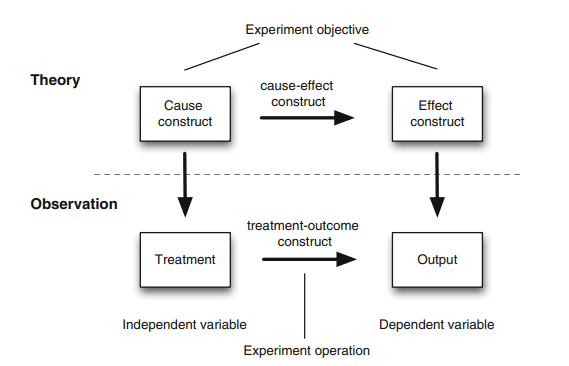
\includegraphics[width=\linewidth]{images/experiment_principles.png}
  \caption{Experiment principles}
  \caption*{Source: Experimentation in Software Engineering}
  \cite{experimentationInSoftwareEngineering}
  \label{fig:experiment_principles}
\end{figure}

This figure shows the theory level and the observation level of an experiment. Theory means that we think that there is some relationship between cause construct and the effect construct. Based on this theory we can construct a hypothesis. On the observation level we test this hypothesis. After the experiment is performed, we are able to observe the results. On the observation level we have some variables, we can consider them "input" variables which are also called independent variables and then we do a treatment on one of those independent variables while trying to fix the levels of other independent variables to make sure they do not modify the result of the experiment. Using this flow, we can observe how the treatment modifies the dependent variable. The illustration of an experiment can be seen in the figure below \ref{fig:experiment_illustration}.

\begin{figure}[h]
\centering
  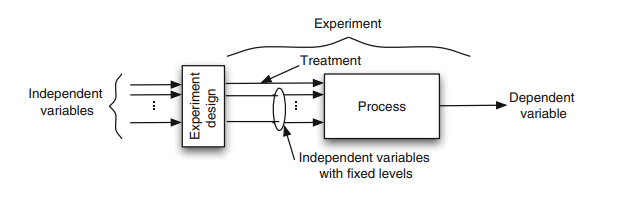
\includegraphics[width=\linewidth]{images/experiment_illustration.png}
  \caption{Illustration of an experiment}
  \caption*{Source: Experimentation in Software Engineering}
  \cite{experimentationInSoftwareEngineering}
  \label{fig:experiment_illustration}
\end{figure}

In our case, we run the experiments in a Dockerized environment to make sure that those independent variables we do not want to do treatment on are fixed.

\subsubsection{Experiment 1}
\label{sec:experiment_1}
In our first experiment we would like to measure how much does it take for a message to reach the AGC from publishing it by the HMI. In our architecture AGC is replicated, which means that we have multiple AGC instances running in parallel. For our experiment we have exactly two AGC instances running. And we do the following treatment: we stop one of the AGC instances for 10 seconds and then we restart it and let it run for 10 seconds, and then stop again for 10 seconds. And we do this as long as we are conducting the experiment. Our hypothesis is that the actual number of AGC instances running does not affect the amount of time needed for the message to reach the AGC.

\subsubsection{Experiment 2}
\label{sec:experiment_2}
In the second experiment we would like to measure how long it takes for the HMI software, which runs in a Docker container, to restart after an unexpected crash. HMI software is designed to be immediately restarted after a crash happens. The treatment here is that we simulate a crash in the HMI software and then measure how much time it takes for the HMI to be up and running again. Our hypothesis is that it should be up in less than 1 second.

\subsection{Measurements}
\label{sec:measurements}
\subsubsection{Experiment 1}
In the case of the first experiment we started the timer when the Start production button was pressed on the HMI screen and stopped the timer when the AGC received the message.

\subsubsection{Experiment 2}
In the case of our second experiment we start the timer when the HMI software started the boot up process and stop the timer when HMI software became fully functional.

\subsection{Pilot test}
\label{sec:pilot_test}
In this section, we are presenting the results we received from the experiments. We only show the first 10 measurements here, but in the scatter plot we display all the measurements we made for both experiments.

\subsubsection{Experiment 1}
After running the first experiment we received the following results: \ref{tab:experiment_1_results}

\begin{table}[h]
    \centering
    \begin{tabular}{ccc}
       \textbf{ID} & \textbf{Elapsed Time (ms)} & \textbf{Ack.} \\ \hline
       1 & 74 & Success \\
       2 & 43 & Success \\
       3 & 39 & Success \\
       4 & 53 & Success \\
       5 & 66 & Success \\
       6 & 41 & Success \\
       7 & 48 & Success \\
       8 & 53 & Success \\
       9 & 41 & Success \\
       10 & 58 & Success \\
       ... & ... & ... \\
    \hline
    \end{tabular}
    \caption{Measurements for Experiment 1 \ref{sec:experiment_1}}
    \label{tab:experiment_1_results}
\end{table}

\subsubsection{Experiment 2}
We got the following results from the second experiment: \ref{tab:experiment_2_results}
\begin{table}[h]
    \centering
    \begin{tabular}{cc}
       \textbf{ID} & \textbf{Elapsed Time (ms)} \\ \hline
       1 & 77 \\
       2 & 77 \\
       3 & 82 \\
       4 & 78 \\
       5 & 81 \\
       6 & 79 \\
       7 & 80 \\
       8 & 82 \\
       9 & 101 \\
       10 & 81 \\
       ... & ... \\
    \hline
    \end{tabular}
    \caption{Measurements for Experiment 2 \ref{sec:experiment_2}}
    \label{tab:experiment_2_results}
\end{table}

\subsection{Analysis}
\label{sec:analysis}
In this section we do the analysis on the results we got after running the experiments. For each experiment, we created a scatter plot on which the elapsed time and the ordinal is shown. After that, we calculated the average elapsed time for both experiments.

\subsubsection{Experiment 1}
For the first experiment we did 44 measurements, and we made a scatter plot to show all the measurements and the elapsed time.


\begin{figure}[h]
\centering
  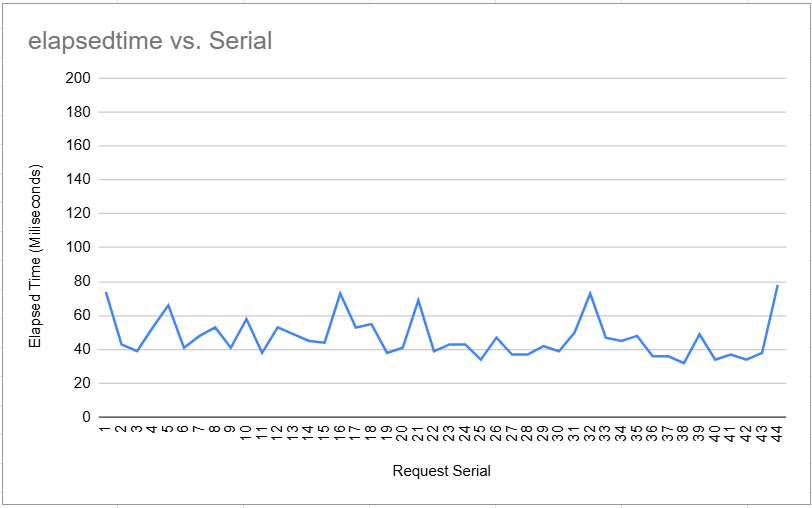
\includegraphics[height=5cm]{images/experiment_1_plot.png}
  \caption{Scatter plot of the first experiment}
  \label{fig:experiment_1_plot}
\end{figure}


In this scatter plot \ref{fig:experiment_1_plot}, it is visible that the Elapsed Time is between 70 and 100 ms. The average Elapsed Time is 47.1 ms. Based on these numbers we can say that the Elapsed Time is not dependent on how many AGC instances are running, which means there is no downtime.
\subsubsection{Experiment 2}
For the second experiment we also did 44 measurements. The figure below shows the scatter plot for the second measurement.

\begin{figure}[h]
\centering
  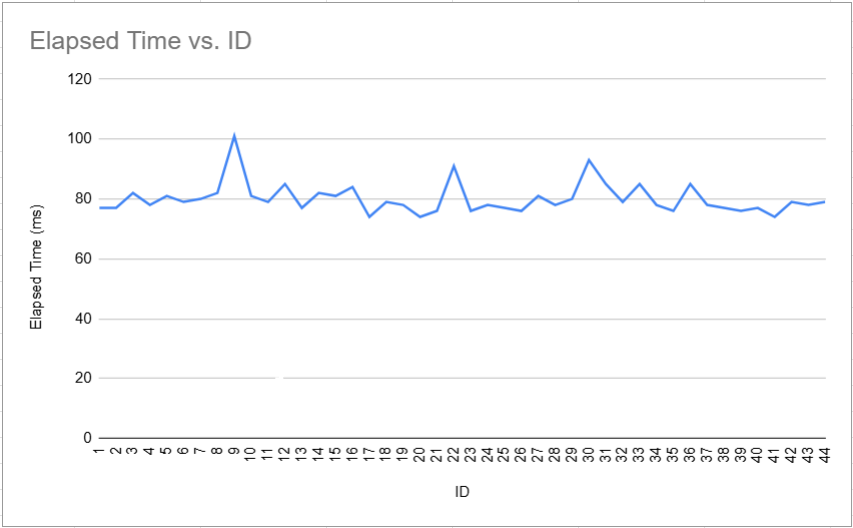
\includegraphics[height=5cm]{images/experiment_2_plot.png}
  \caption{Scatter plot of the first experiment}
  \label{fig:experiment_2_plot}
\end{figure}

In the case of the second experiment the Elapsed Time is between 70 and 100 ms, and their average is 80.1 ms which is significantly less than 1 second stated in our requirements.